\documentclass[xcolor=table]{beamer}
\usepackage{beamerthemeCambridgeUS}
\usepackage{color}  % for \textcolor{red}{blah}
\usepackage{graphicx}
\usepackage{array}
\usepackage{subfigure}
\usepackage{multicol}
\usepackage{verbatim} % for \begin{comment}
\usepackage{lipsum}


\newcommand\Fontvi{\fontsize{6}{7.2}\selectfont}


\newenvironment{packed_enum}{
\begin{enumerate}
  \setlength{\itemsep}{1pt}
  \setlength{\parskip}{0pt}
  \setlength{\parsep}{0pt}
}{\end{enumerate}}

\newenvironment{packed_item}{
\begin{itemize}
  \setlength{\itemsep}{1pt}
  \setlength{\parskip}{0pt}
  \setlength{\parsep}{0pt}
}{\end{itemize}}

\usetheme{CambridgeUS}

\title{Discrete Mathematics}
\author[Geoffrey Buhl]{Geoffrey Buhl \\ \texttt{geoffrey.buhl@csuci.edu}}
\institute[CSUCI]{California State University Channel Islands}
\date{week 3 class 2}

\def \vec{{\rm vec}}
\newtheorem{conjecture}[theorem]{Conjecture}
\newtheorem{explanation}[theorem]{Explanation}


\begin{document}

%\frame{\titlepage}

%\section[Outline]{}
%\frame{\tableofcontents}

\section{Class 5 - Binomial Coefficients and the Binomial Theorem}


\frame
{
  \frametitle{Choosing with order not mattering and repetition not allowed}

Class Session Goals:
\begin{packed_enum}
\item Present Binomial Coefficients, Pascal's Triangle, and Unordered Selection Table
\item Practice turning patterns into expression and Formulas
\item Present Combinatorial Proof of Pascal Triangle Identity
\item Present Induction Proof of Binomial Theorem
\end{packed_enum}

}


\frame
{
  \frametitle{Unordered Selections}

The number of ways to choose $k$ times from $n$ objects where order does not matter and repetition is not allowed is  $$\binom{n}{k}=\frac{n!}{(n-k)!k!}$$ for $n$ and $k$ and $n \ge k$ and 0 if $n <k$.
\vfill


}

\frame
{
  \frametitle{Table of Unordered Selections}
Values of $\binom{n}{k}$ for $n=0,\ldots, 5$ and $k=0,\ldots, 5$.\vfill

$$
\begin{array}{rcccccc}
 & k=0 & k=1 & k=2 & k=3 & k=4 & k=5\\
n=0: &1 & 0 & 0 & 0 & 0& 0 \\
n=1:&1 & 1 & 0 & 0 & 0 & 0\\
n=2:&1 & 2 & 1 & 0 & 0 & 0\\
n=3:&1 & 3 & 3 & 1 & 0 & 0\\
n=4:&1 & 4 & 6 & 4 & 1 & 0\\
n=5: &1 & 5 & 10 & 10 & 5 & 1\\
\end{array}
$$
\vfill
}

\frame
{
  \frametitle{Binomial Expansion}

The expression  $(x+y)^n$ is called a binomial expansion. The coefficients of monomials $x^ky^{n-k}$ are called binomial coefficients.  Below are binomial expansion for $n=0,\ldots, 5$\vfill

$$
\begin{array}{c}
 1 \\
 x+y \\
 x^2+2 x y+y^2 \\
 x^3+3 x^2 y+3 x y^2+y^3 \\
 x^4+4 x^3 y+6 x^2 y^2+4 x y^3+y^4 \\
 x^5+5 x^4 y+10 x^3 y^2+10 x^2 y^3+5 x y^4+y^5 \\
\end{array}
$$
\vfill
}

\frame
{
  \frametitle{Pascal Triangle}
The first six rows of Pascals Triangle with the intial row being row 0. \vfill

\begin{tabular}{rccccccccccc}
$n=0$:&&    &    &    &    &  1\\\noalign{\smallskip\smallskip}
$n=1$:&&    &    &    &  1 &    &  1\\\noalign{\smallskip\smallskip}
$n=2$:&&    &    & 1 &    &  2 &    &  1\\\noalign{\smallskip\smallskip}
$n=3$:&&    &  1 &    &  3 &    &  3 &    &  1\\\noalign{\smallskip\smallskip}
$n=4$:&&  1 &    &  4 &    &  6 &    &  4 &    &  1\\\noalign{\smallskip\smallskip}
$n=5$:&1&  &5 &    &10 &    &  10 &    &  5 &    &  1\\\noalign{\smallskip\smallskip}
\end{tabular}
\vfill
}

\frame
{
  \frametitle{Activity}

In small groups, work on the ``Patterns and Formulas in Pascals Triangle'' worksheet. The goals of this worksheet are to:

\begin{packed_enum}
\item Identify Patterns in Pascals Triangle
\item Create mathematical equations that represent these patters
\end{packed_enum}


}

\frame
{
  \frametitle{Pascal's Triangle}



\begin{figure}[h]
  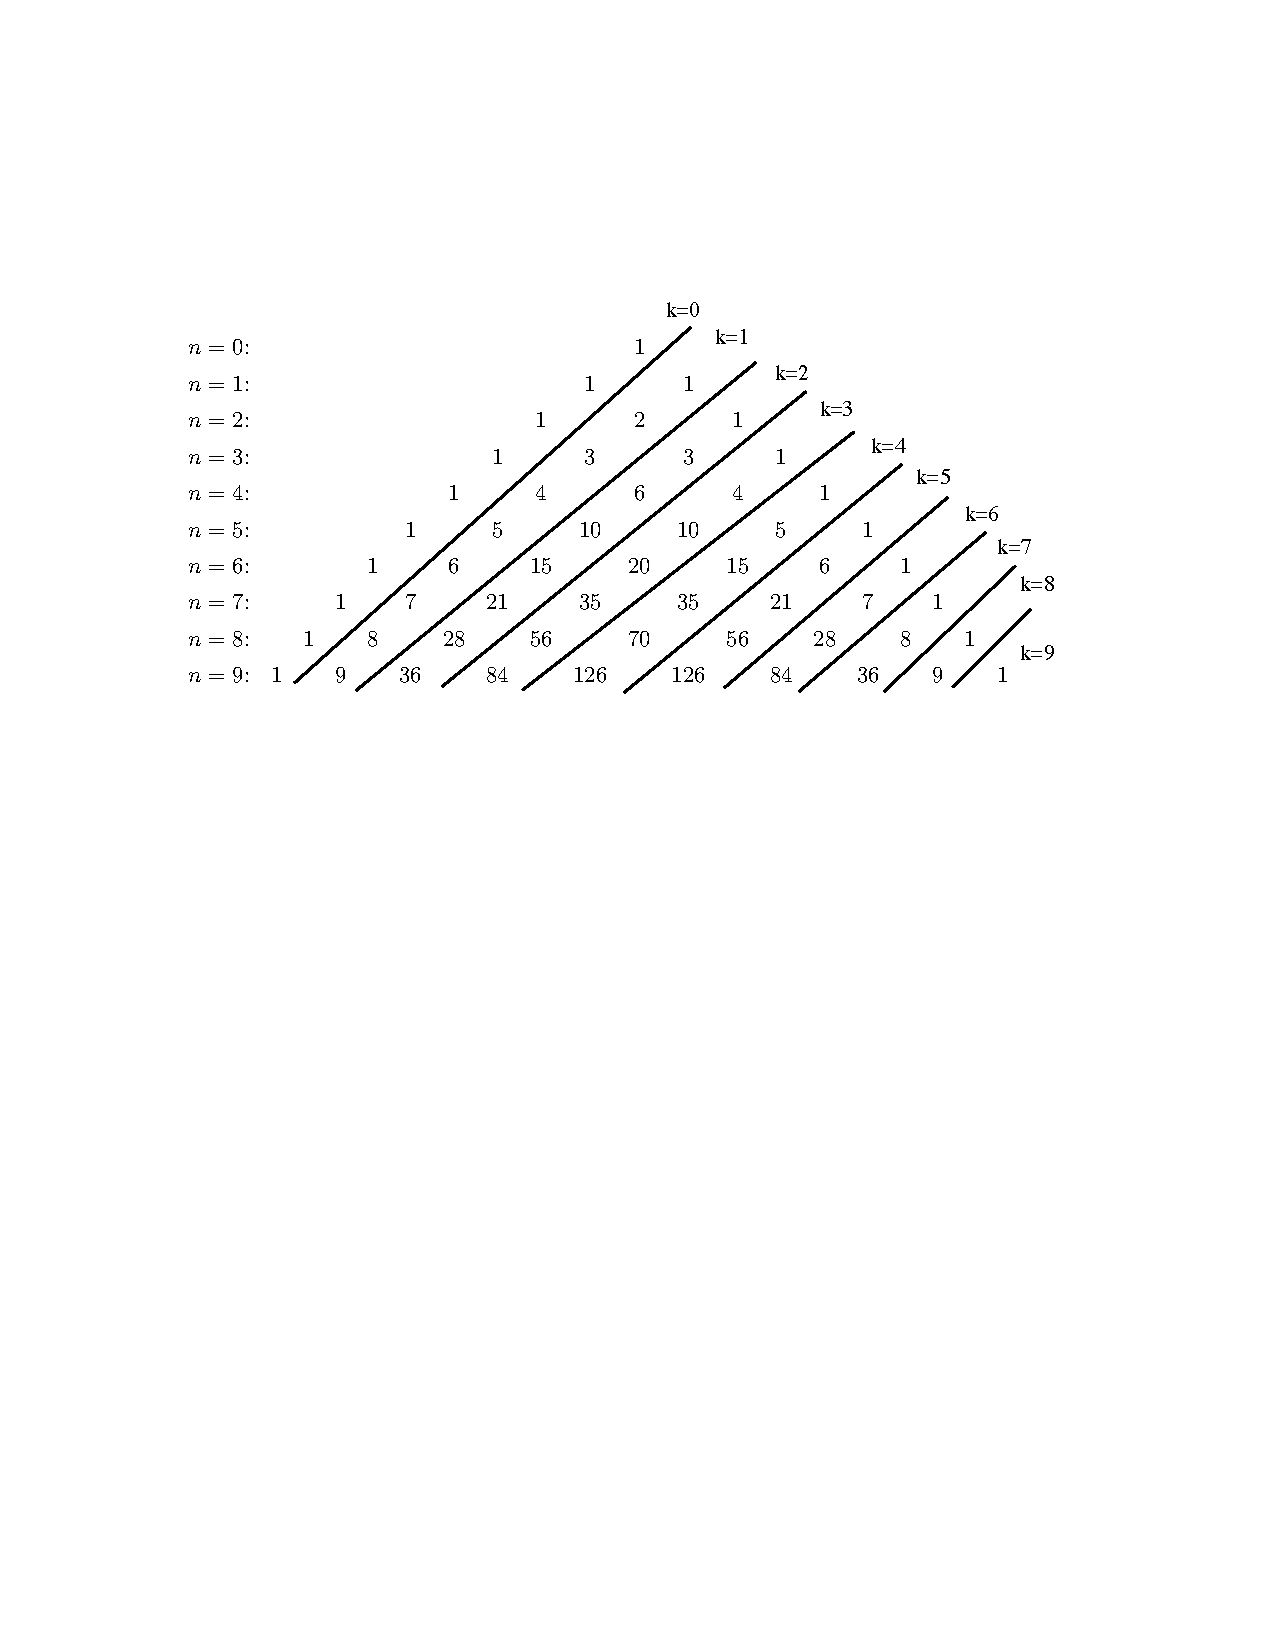
\includegraphics[scale=.4]{triangel with diagonals.jpg}
 \end{figure}


}


\frame
{
  \frametitle{Pascal's Triangle}
\footnotesize


\begin{tabular}{rcccccccccccccccccc}
&&&&&    &    &    &    &  1\\\noalign{\smallskip\smallskip}
&&&&&   &    &    &  1 &    &  1\\\noalign{\smallskip\smallskip}
&&&&&    &    &  \cellcolor{green!25}1 &    & \cellcolor{green!25} 2 &    & \cellcolor{yellow!25}  1\\\noalign{\smallskip\smallskip}
&&&&&    &  1 &    & \cellcolor{green!25} 3 &    &  \cellcolor{yellow!25}3 &    &  1\\\noalign{\smallskip\smallskip}
&&&& & 1 &    &  4 &    &  \cellcolor{yellow!25}6 &    &  4 &    &  1\\\noalign{\smallskip\smallskip}
&&&&1&  &5 &    &  10 &    &  \cellcolor{yellow!25}10 &    &  5 &    &  1\\\noalign{\smallskip\smallskip}
&&&1&  &6 &    &  15 &    &  20 &    &  15 &    &  6 &&1\\\noalign{\smallskip\smallskip}
&&1&  &7 &    & \cellcolor{blue!25} 21 &    &  35 &    &  35 &    & \cellcolor{blue!25} 21&&7&&1\\\noalign{\smallskip\smallskip}
&1&  &8&    &  28 &    &  56 &    & 70 &    &  56&&28&&8&&1\\\noalign{\smallskip\smallskip}
\end{tabular}

}


\begin{frame}
\frametitle{Activity's Formulas}

\begin{tabular}{l<{\onslide<2->}l<{\onslide}}
{\bf Pascal's Triangle Identity}: &$\binom{n-1}{k}+\binom{n-1}{k-1}=\binom{n}{k}$\\
{\bf Left-Right Symmetry Formula}: &$\binom{n}{k}=\binom{n}{n-k}$\\
{\bf Hockey Stick Formula} &$\sum_{i=0}^{k}\binom{n+i}{n}=\binom{n+k+1}{n+1}$\\
{\bf Sum of Rows Formula} & $\sum_{k=0}^{n}\binom{n}{k}=2^n$\\
{\bf Alternating Sum of Rows Formula} &$\sum_{k=0}^{n}(-1)^k\binom{n}{k}=0$\\
\end{tabular}

\end{frame}

\frame
{
  \frametitle{Pascal's Triangle Identity}

$$\binom{n-1}{k}+\binom{n-1}{k-1}=\binom{n}{k}$$ \vfill
or
$$\binom{n}{k}+\binom{n}{k-1}=\binom{n+1}{k}$$
By substituting $n+1$ in for $n$. \vfill

This explains the connection between the table of unordered selection numbers and Pascals Triangle.
}

\frame
{
  \frametitle{Binomial Theorem}

{\bf Binomial Theorem}:For $n\ge 0$, $(x+y)^n= \sum^{n}_{k=0}\binom{n}{k}x^ky^{n-k}$.\vfill
This explains the connection between the table of unordered selection numbers and Pascals Triangle.
}

\begin{comment}
\frame
{
  \frametitle{Puzzle}

\begin{tabular}{rccccccccc}
$n=0$:&1    &    &    &    &  \\\noalign{\smallskip\smallskip}
$n=1$:&1    &1    &    &   &    &  \\\noalign{\smallskip\smallskip}
$n=2$:&2    &1    &    &   &    &  \\\noalign{\smallskip\smallskip}
$n=3$:&1    &1    &  1 &    2&   &    &  \\\noalign{\smallskip\smallskip}
$n=4$:& 3   &  1 &1    & 2 &    &   &    &  \\\noalign{\smallskip\smallskip}
$n=5$:&  2 &  1  &  1 &  2  &  1 &   3 &   &    &  \\\noalign{\smallskip\smallskip}
$n=6$:&  3 &  1  & 2 &  2  &  1 &   3 &   &    &  \\\noalign{\smallskip\smallskip}
$n=7$:&  2 &  1  & 2 &  2  &  2 &   3 &   &    &  \\\noalign{\smallskip\smallskip}
$n=8$:&  1 &  1  & 4 &  2  &  1 &   3 &   &    &  \\\noalign{\smallskip\smallskip}
$n=9$:&  3 &  1  & 1 &  2  &  1 &   3 &  1 &   4 &  \\\noalign{\smallskip\smallskip}

What's the next line?

\end{tabular}
}
\end{comment}

\end{document}



